\section{Validation}

Cette partie vise à tester et valider le comportement des blocs fonctionnels.
Elle se positionne sur la pente remontante du cycle en V.

\subsection{Test unitaire}

\subsubsection{Solutionneur de priorités}
Le bloc solutionneur de priorités prend en entrée les 15 sources d'interruptions provenant des autres périphériques et le registre des priorités.
Il doit, à partir de cela, présenter en sortie le numéro de l'interruption active la plus prioritaire.
La gestion des interruptions n'étant pertinente, dans un processeur, que si la latence est réduite au minimum.
C'est pourquoi nous avons fait le choix de concevoir une solution asynchrone qui assure sa fonction en moins d'un cycle horloge.
La simulation suivante ne possède donc pas d'horloge.
Les deux conditions de priorité sont testées.
La première, si deux interruptions sont valides au même instant, c'est l'identifiant de la plus prioritaire au regard du registre \texttt{CTRL\_IT\_PRIO\_N} qui est placé en sortie.
La seconde, correspond au cas particulier où deux interruptions de même priorité seraient actives simultanément.
Dans cette situation, c'est l'identifiant le plus grand qui est sélectionné.
\begin{figure}[H]
    \centering
    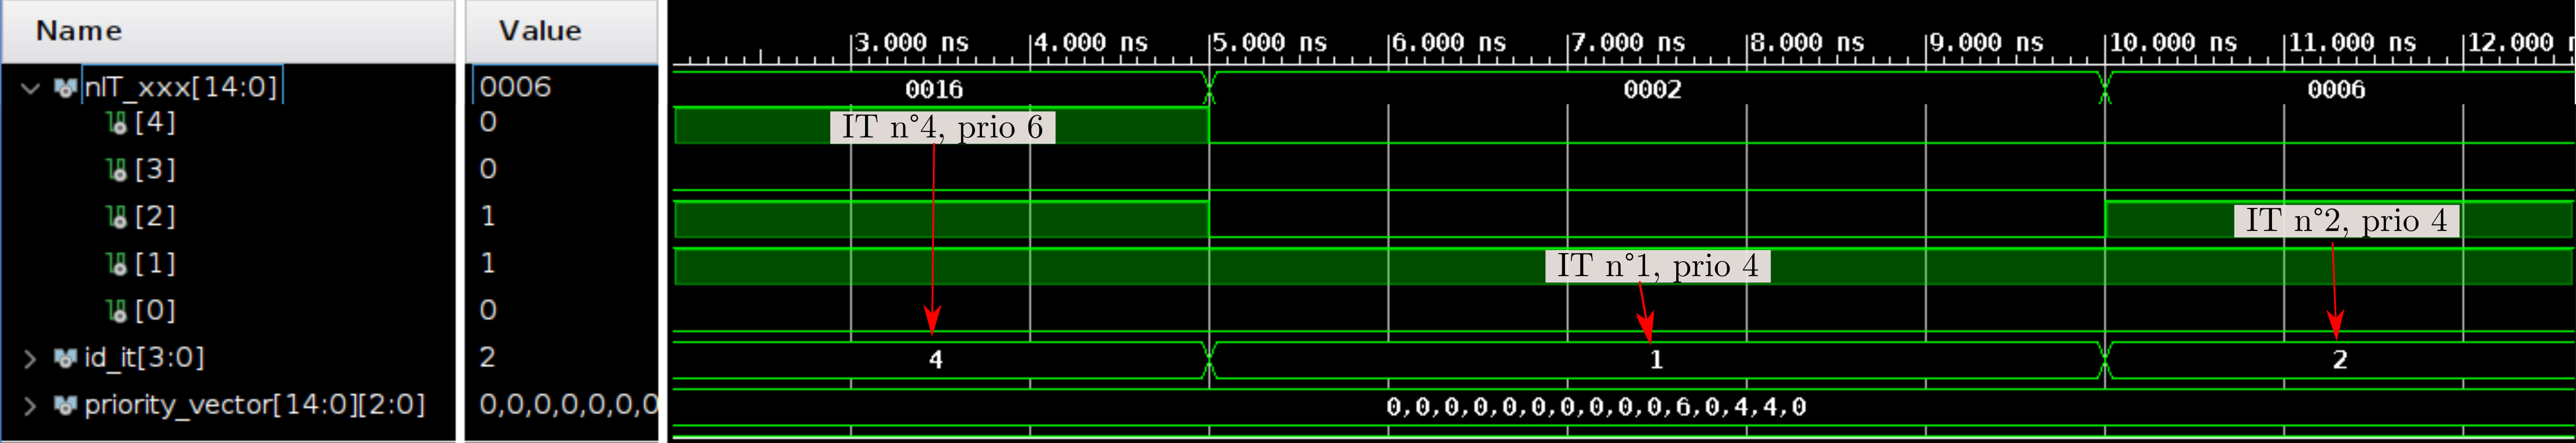
\includegraphics[width=1.1\linewidth]{chrono_priority_solver.draw.png}
    \caption{Chronogramme validation solutionneur priorité}
    \label{fig:chrono_prio_solv}
\end{figure}
La figure \ref{fig:chrono_prio_solv} illustre le résultat du bloc solutionneur priorité lorsqu'il est soumis à une banc de test.
Bien que les stimulus d'entrée prennent un grand nombre de valeurs dans la simulation originale, seul trois cas sont présentés.
Les priorités sont inchangées au cours de ce test et leur valeur sont $IT_4=6$, $IT_1=4$, $IT_2=4$.
Dans le premier, trois interruptions sont valides simultanément.
C'est l'identifiant 4 qui est placé en sortie, car sa priorité est de 6 contre 4 pour deux les autres.
Dans le deuxième cas, seul une interruption est valide, il n'y a pas d'arbitrage, la valeur 1 est visible en sortie.
Le dernier illustre la situation particulière où les 1 et 2 ont la même priorité.
C'est donc le numéro 2 qui prend la main.
Le chronogramme atteste du bon fonctionnement du bloc solutionneur de priorités.


\subsubsection{Masque}

Le bloc masque permet à l'utilisateur d'inhiber les sources d'interruption de son choix.
Il prend en entrée les 15 sources d'interruption et le registre \texttt{CTRL\_IT\_MSQ}.
Son fonctionnement est plutôt simple.
Le registre est d'abord inversé bit à bit puis un ET logique est appliqué avec les sources.
Seuls, les bits non masqués sont transmis au bloc suivant.
\begin{figure}[H]
    \centering
    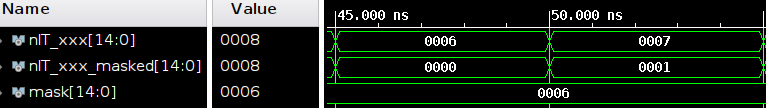
\includegraphics[width=0.8\linewidth]{chrono_mask.png}
    \caption{Chronogramme validation bloc masquage}
    \label{fig:chrono_mask}
\end{figure}
La figure \ref{fig:chrono_mask} illustre deux exemples du bloc masquage soumis aux stimulus du banc de test.
Le masque est affecté à la valeur 6, $(110)_2$, pendant les deux situations.
Les sources 1 et 2 sont donc  masquées.
Dans le premier cas, ces deux sources sont actives, elles sont donc inactivées sur la sortie.
Dans un second temps, la source 0 émet une demande d'interruption.
Cette dernière n'étant pas masqué, elle est conservée seule.
